\documentclass[11pt,letter]{article}
\usepackage[top=1.00in, bottom=1.0in, left=1.1in, right=1.1in]{geometry}
\renewcommand{\baselinestretch}{1.1}
\usepackage{graphicx}
\usepackage{natbib}
\usepackage{gensymb}
\usepackage{amsmath}
\usepackage{lineno}
\usepackage{xr-hyper}
\externaldocument{limitingcues_supp}

\def\labelitemi{--}
\parindent=0pt

\usepackage{Sweave}
\begin{document}
\bibliographystyle{/Users/Lizzie/Documents/EndnoteRelated/Bibtex/styles/besjournals} % change to pnas to count refs
\renewcommand{\refname}{\CHead{}}
\begin{flushright}
Version dated: \today
\end{flushright}
\bigskip
\noindent RH: Interactive cues \& phenology
% put in your own RH (running head)

\bigskip
\medskip
\begin{center}

% Insert your title:
\noindent{\Large {\bf Integrating experiments to predict the interactive effects of temperature and photoperiod on spring phenological responses to warming}}\\ % OR How interactive cues will shape non-linear climate change responses ? 
% Concept paper on understanding interactive cues and climate change (with growth chamber studies) 
\bigskip

\noindent {\normalsize \sc
E. M. Wolkovich$^{1,2}$, C. J. Chamberlain$^{1,2}$, D. M. Buonaiuto$^{1,2}$, A. K. Ettinger$^{3}$ \\ \& I. Morales-Castilla$^{5}$}\\ % The lab in 2017 -- Lizzie, Ailene, Cat, Dan, Nacho

\noindent {\small \it
$^1$ Forest \& Conservation Sciences, Faculty of Forestry, University of British Columbia, 2424 Main Mall, Vancouver, BC V6T 1Z4\\
$^2$ Arnold Arboretum of Harvard University, 1300 Centre Street, Boston, Massachusetts, 02131, USA\\
$^3$ Organismic \& Evolutionary Biology, Harvard University, 26 Oxford Street, Cambridge, Massachusetts, 02138, USA\\
$^4$ The Nature Conservancy, 74 Wall Street, Seattle, Washington USA\\
$^5$ Global Change Ecology and Evolution Group, Department of Life Sciences, University of Alcal\`a, Alcal\`a de Henares 28805, Spain}
\end{center}
\medskip
\noindent{\bf Corresponding author:} Lizzie, see $^{3}$ above ; E-mail: e.wolkovich@ubc.ca\\


% 229 words; XX refs on 3 December 2021
\begin{abstract} Climate change has advanced plant phenology globally 4-6 days per $\degree$C on average, with some species shifting much more. Such shifts have been some of the most reported and predictable biological impacts of rising temperatures. Yet as climate change has marched on, phenological shifts have appeared muted over recent decades---failing to match simple predictions of an advancing spring with continued warming. The main hypothesis for these changing trends is that interactions between spring phenological cues---long-documented in lab environments---are playing a greater role in natural environments due to climate change. Here we argue that accurately linking shifts observed in long-term data to underlying phenological cues is currently stymied by biases in observational studies and limited study of interactions in experiments. We synthesize seven decades of research in controlled environments to quantify how much phenological cue-space has been studied and how treatments compare to shifts in cues caused by climate change. We find that most studies focus on one cue, and often study differences in cues far beyond those predicted with climate change, limiting our ability to predict non-linear responses. We outline how greater integration of controlled environment experiments  with long-term data and insights from physiology, alongside a new generation of lab experiments could transform our fundamental understanding of phenology and improve forecasts of shifting phenology.  % Change tone here to -- we need better understanding of these other cues if we want to understand shifts across space and time. 
\end{abstract}

% \noindent \emph{Main message (and, really, it's important):} If you want to project climate change impacts, you need to focus on relevant changes in all three cues. The relevant changes part is about comparing cues, the all three cues is about interactive cues.
% Old abstract (2019 one):
% ... most predictable biological impacts of climate change. This predictability comes from decades of research, which have outlined the major cues that drive most studied plant phenology: temperatures (including spring warming and winter chilling) and daylength. Further simplifying predictions, spring temperatures are often the dominant cue in nature, making linear models of heat sums often excellent at predicting interannual variation in phenology. Yet as climate change has marched on, new research has uncovered possible failures to predict the current observed changes; increasingly, phenological shifts appear more muted over recent decades, or in certain locations. Here we argue that some of these inaccurate predictions are due to simple models that neglect to consider other major cues---especially winter chilling and daylength, which moderate and shape plant phenological responses to spring warming. We highlight how over 70 years of research in controlled environments can improve predictions for when, where and how the interactive effects of other cues will impact simple linear predictions. Finally, we discuss how a new generation of controlled environment experiments could rapidly improve our predictive capacity for woody plant phenology in coming decades.  

\noindent \emph{Keywords:} phenology, climate change, spring warming, chilling, forcing, daylength, photoperiod, non-linear responses, leafout, budburst\\

\newpage
\linenumbers
\section{Main text} % Currently about 4422 words with embedded refs; estimated words when using numbered refs (about 375 words in in-text citations)
Shifts in spring plant phenology are one of the most reported and predictable changes with climate change. Decades of research have documented advancing budburst, leafout and flowering with climate change \citep{delpierre2009, yu2010,Ellwood2012,jochner2013,hereford2017}, especially in temperate systems where long-term records highlight how humans have altered the timing of spring \citep{Schwartz:1997nn,Menzel2003a,menzel2006}. Recently, however, these advances have appeared to slow \citep{fu2015} or even reverse \citep{yu2010}---failing to match simple predictions of an advancing spring with continued warming \citep{Ellwood2012}. The main hypothesis for this failure is that spring warming---which most observational studies focus on---is no longer the only environmental cue that matters to predicting responses to warming \citep{chuine2016,gauzere2019}.\\

Despite the strong focus of spring phenology research on spring temperatures, increasing evidence suggests a more complicated underlying physiology for most plant species \citep[e.g.,][]{zohner2016,gauzere2019,ettinger2020}. For many species three major cues underlie spring phenology: chilling (cool temperatures, generally occurring in the fall and winter), forcing (warm temperatures, generally occurring in the late winter and early spring), and photoperiod (daylength). \\

Together, chilling, forcing and photoperiod may produce non-linear responses that many current methods do not predict, but observational studies have reported recently \citep{fu2015}. Predicting these non-linearities is a common goal in plant phenology research today \citep{gusewell2017,martlusch2017,gauzere2019,chen2019,keenan2019}, but has been slowed by data gaps and the complexity of spring phenological cues. While each cue alone may be linear in the mid-range of values, extremely high or low values can produce threshold responses \citep{major1980,Heide:1993,Partanen:1998aa,Singh:2017,rinne2018}. Such extreme values are likely uncommon in natural environmental regimes.\\

Most hypotheses for the observed decline instead invoke the interaction between cues to produce non-linear responses to warming. Yet estimating the effect of interactions from observational data, where cues themselves often covary, may produce spurious results \citep{ettinger2020}. In contrast, controlled environment (e.g., growth chamber) studies are designed to understand and estimate multiple cues, and can tease out their interactive effects. \\ % are designed to understand nonlinear responses to warming, both in one cue alone and through the interaction of multiple cues.

Here we argue that using controlled environmental studies to estimate cue interactions is critical to robust forecasts of phenological shifts with climate change. Such studies have been conducted for over 70 years, but they have rarely been reviewed and are often poorly integrated into the current phenological literature on climate change \citep[e.g.,][]{fu2015,richardson2018}. To address this gap, we synthesize these studies (Fig. \ref{fig:datamap}) to quantify how much of the cue-space (i.e., the possible range of each cue and interactions across cues) has been studied and how treatments compare to shifts in cues caused by climate change. Based on this, we suggest a cross-disciplinary path forward where advances in physiology, greater integration of controlled environment studies with forecasting, and multi-species modeling can yield more robust predictions.\\

Given our aim to improve understanding of current trends and forecasts we focus on early vegetative phases (budburst and leafout), which are critical to plant growth and carbon storage, have shifted most with climate change \citep{Cleland:2007or,IPCC:2014sm}, and have been studied the most in experiments (see Supporting Information). Our review concentrates on woody species phenology, where most research on budburst and leafout has occurred. Most of our conclusions and suggested approaches, however, could be adapted to non-woody species and other phenophases with similar underlying interactive cues. 

\subsection{Why observational studies are not enough to robustly estimate cues}
The first step towards robust phenological predictions is accurate measurements of chilling, forcing and photoperiod cues. Recently, efforts have focused on estimating these cues from long-term observational data \citep{Luedeling2009,lued2013diff}. Yet observational studies may struggle to robustly estimate any of the three major cues due to two types of statistical issues. First, in most observational data these cues correlated: forcing increases alongside longer photoperiods \citep{sarahailene2020}, and changes to chilling and photoperiod cues with warming predict the same response---later spring phenology. Approaches that attempt to disentangle some of these correlations, such as leveraging trends across elevation or latitude, may run afoul of other correlations \citep[][]{tansey2017}. Second, most observational studies focus on linear models of each cue, often without interactions between cues \citep{visser2001,polgar2014}. Even when interactions are invoked to explain declining responses to warming, they are often not estimated \citep[e.g.,][]{fu2015,asse2018}.\\

In contrast to observational studies, controlled environment studies can manipulate each cue independently. By experimentally decoupling cues, they can thus tease out interactions between them. Perhaps unsurprisingly then, most of our fundamental understanding of these cues comes from controlled environment studies.\\

Controlled environment studies have shown that chilling, forcing and photoperiod cues together determine the transition from dormancy to growth (usually first observed as budburst) each year for most temperate woody species \citep{vanderschoot2014,chuinearees,Singh:2017,ettinger2020,chang2021}. Chilling and forcing cues are generally understood to be accumulation processes, where plants integrate chilling and forcing experienced over time to meet a threshold value at which they can budburst, leafout or flower \citep{Chuine2000}. In contrast, photoperiod is generally not considered an integral cue, but one evaluated daily \citep{Singh:2017}. In practice, these two types of processes are often abstracted into the effects of average experienced values (mean temperature or daylength), generally over some temporal window in long-term data \citep[e.g.,][]{Wolkovich:2012n,fu2015}, or by holding temperatures and light regimes more constant in experiments \citep[e.g.,][]{Worrall:1967aa,Heide:1993,Heide:1993a,Skuterud:1994aa}. \\ % Several recent reviews have focused on the cellular and molecular aspects of this critical transition \citep{vanderschoot2014,Singh:2017,chang2021}, thus we provide only a very brief review of each cue. 

Climate change is likely altering each of the three cues. Most notably to date, warming increases forcing, with more rapid---and thus greater---shifts at higher elevations and in the arctic \citep{IPCC:2014sm}. Warming likely also translates into shifts in chilling, which long-term observational studies have repeatedly suggested may already be occurring \citep{fu2015,piao2017}, but such estimates are complicated by our limited understanding of chilling (see Supporting Information). Additionally, the relevant photoperiod a plant experiences at critical physiological points may change dramatically with warming \citep[despite that an environment's photoperiod does not shift with climate change,][]{ospreephoto}. In particular, increases in chilling and/or forcing, which could alone produce much earlier budburst, may be offset by short photoperiods that delay budburst \citep{gauzere2019}. \\ %Similarly, long photoperiods can lead to budburst sooner than predicted solely by low chilling or forcing conditions \citep{Nienstaedt:1966aa,Myking:1995,Partanen:1998aa}.

Researchers hypothesize that these shifts---in forcing, chilling and photoperiod experienced near the time of an event---produce non-linearities in plant responses to warming. While a growing number of observational studies have attempted to document non-linear shifts in phenology due to interactive cues \citep{fu2015,gauzere2019}, understanding exactly when cues cause non-linearities may be more complicated than often presented (Fig. \ref{fig:intxncues}), and almost always relies on knowledge gained from controlled environment studies \citep[e.g.,][]{fu2015,richardson2018,gauzere2019}.

\subsection{Interactions alone are unlikely to produce non-linearities with warming}
Interactions are well-documented in controlled environment studies. Multiple studies now show that the threshold of forcing needed for budburst depends on the sum of chilling over the fall and winter and also the photoperiod experienced in the spring \citep[e.g.,][]{zohner2014,flynn2018}. Higher forcing is generally needed given lower chilling (Fig. \ref{fig:gddbyutah}) and shorter photoperiods \citep{Basler:2014aa,fu2019}. This yields a sub-additive interaction of forcing x chilling and forcing x photoperiod, where high values of both cues together produce a more muted response than would be expected from examining either cue alone.\\

These interactions alone may produce a more muted response but they do not necessarily produce non-linearities (Fig. \ref{fig:intxncues}). Instead most hypotheses for non-linear responses tacitly require both the interaction of cues and covarying shifts in cues with warming to produce non-linearities. For example, if some species have a critical photoperiod for budburst and warming leads to forcing cues being met before the critical threshold---effectively shifting both the forcing and photoperiod cues---then we would expect incomplete or highly delayed budburst \citep{Singh:2017,rinne2018}. Alternatively, the threshold could be crossed in the opposite direction. In this example pre-climate change conditions would have caused budburst to occur at the extreme values of some cues, but warming could push budburst into values where responses are more linear.  This is the mechanism often suggested for declining responses to warming in some temperate trees \citep{fu2015,piao2017,gauzere2019}, specifically that plants previously accumulated sufficient chilling such that forcing was the dominant cue---whereas warming has now reduced chilling such that more forcing is needed for budburst \citep[producing an overall muted effect when estimated as change in days per $\degree$C, see][for one example]{fu2015}. As this example highlights, however, changes in a single cue are unlikely to occur without additional effects on other cues---complicating how well we can understand them in long-term data without robust understanding of the exact cue requirements from other methods.

% Thus, while simple linear interactions between cues may not alone produce non-linearities, they quickly become non-linear when changes in cues occur together.  Predicting these non-linearities, however, requires a refined understanding of the interaction between cues and whether there are critical inflection points that may be crossed with continued warming. % These complexities highlight how we need greater efforts to tease out how each cue works alone and interactively. 

% We outline how the three major phenological cues---forcing, chilling and photoperiod---can produce non-linearities and how they will shift in coming decades with anthropogenic climate change. \\
\subsection{Forecasting non-linear responses: Do we have the necessary data?} % ... with controlled environment experiments
Controlled environment studies can help predict non-linear responses by allowing researchers to examine the effects of one cue with the others held constant, and examine interactive effects---given the appropriate study design. Such experiments may be especially useful for forecasting if they contain enough variation in treatments to capture precisely where non-linearities occur, and are designed across a range of levels relevant to current versus future conditions \citep{shen2015}. Indeed, one of the major advantages of experiments is that they allow treatments outside of the historical range of a species' (or region's) climate---an option observational data cannot provide. \\

To understand how valuable currently available data may be to forecasting, we reviewed controlled environment studies over the last seven decades, quantifying the range of treatments and how they compare to current and future conditions. These studies were rarely conducted for climate change research, and most often done for reasons of fundamental or applied science (e.g., horticulture or forestry). Yet they are some of the best available data for how plants respond to the environment and thus a critical resource for climate change research today.\\

\emph{How studies and their experimental treatments vary globally}\\
Controlled environment studies have been conducted with 226 woody species across the globe, with the majority of papers reporting research occurring in Europe (54 of 84 papers; and 93 of 136 studies across papers; a study is a unique experiment within a paper), followed by North America (22 papers and 32 studies, Fig. \ref{fig:datamap}, Table \ref{tab:ref}). Most studies manipulate one cue though studies of two or three cues have occurred in almost every decade (Fig. \ref{fig:ts}). Across study designs, chilling was the most commonly studied cue (69\% of 117 studies that manipulated at least one cue; with roughly half of these studies---47\%---using outdoor chilling through multiple field sampling dates), followed by forcing and photoperiod (43\% and 40\%, respectively). \\

Studies have covered only a small portion of cue-space (especially for experimentally applied chilling, Fig. \ref{fig:heatmaps}), with certain levels of cues much more common than others. Photoperiods of 12, 16} and 24} hours represented 65\% of all photoperiod treatments, while almost half (47\%) of all forcing treatments were 10, 20 or 25$\degree$C. This suggests we have greater inference at these cue levels, but also more limited understanding beyond them, which could limit forecasting. Chilling treatments were far more varied. Of the studies that reported chilling temperatures, 4$\degree$C was the most common (at only 14\% of all studies), followed by 0$\degree$C  and 3$\degree$C (at 11\% and 9\%, respectively).\\

The levels of cues also varied across latitude with a general trend toward examining more extreme values at higher latitudes (see Fig. \ref{fig:lat}). This trends appears related to latitudinal clines in the environment---higher latitudes experience colder temperatures and longer photoperiods, and see similar shifts in their controlled environment study designs. But this trend also introduces a bias in results, as any comparisons of studies from lower and higher latitudes are also comparing a different range of cues. \\
% See countintxns.R 
% Need to add: 
% (1) Table of all analyses to supp
% (2) Say something about material (seeds/saplings/cuttings)? Can we tie to relevance of predicting future forest communities or such?

\emph{How studies manipulate cues}\\ % may be especially insightful for forecasting, ... Experiments that manipulate multiple cues are the only robust way to estimate interactive effects, but they are less common than single cue studies.
Single-cue studies were the most common (65 studies), with most manipulating chilling  (41 studies), followed by 14 manipulating photoperiod and 10 manipulating forcing (Fig. \ref{fig:heatmaps}). Single cue studies can be valuable for defining potential non-linearities in one cue, but are difficult to use for forecasting as they prevent understanding interactions among cues or comparisons of which cues dominate phenological responses. \\
% Nacho says: I know you asked us not to include refs from the group, but just in case, citing Flynn and Wolkovich would seem appropriate there.
% Of the studies manipulating chilling, 14 used only field conditions for chilling treatments.

To robustly test for interactions studies must use an experimental design that includes most or all combinations of all levels of cues studied (factorial design). Of the studies manipulating at least one cue, roughly a third additionally manipulated another cue in a factorial design (37\% or 43 studies), with the studies almost evenly split across all possible two-way interactions (14 studies of photoperiod x chilling, followed by 13 studies of forcing x chilling, followed by 12 studies of photoperiod x forcing; 4 studies did not include an interaction; studies with chilling used field chilling more often than chilling applied in controlled environments, 16 versus 11 studies). \\
%  Studies examining photoperiod or forcing crossed with experimental chilling treatments (either through changes in temperature or days of chilling) were much less common (6 studies for photoperiod and 5 studies for forcing). \\

Studies examining three cues directly were rare: we identified only three studies examining all three cues at once. Two of these were on \emph{Picea abies} \citep{Worrall:1967aa,Sogaard:2008aa}, and the other on \emph{Betula pendula} \citep{Skuterud:1994aa}. A slightly larger set of studies (5 studies from 4 papers) examined three cues indirectly---manipulating photoperiod and forcing in controlled environments but equating chilling with sequential removal of tissue from the field---for 11 species \citep{Schnabel:1987aa,Heide:1993,Partanen:1998aa,Basler:2014aa}. \\
% I think we need to add what the interactive studies found -- did they all find interactions? 
% "okie11_exp2"  -- Peach, doesn't really cross forcing (mainly chill x photo)   "worrall67_exp 3" (this paper coolly opens with "As has been repeatedly emphasized in the literature, discussions of dormancy in woody plants are often misleading because of the lack of a standard nomenclature.") and "sogaard08_exp2" .... both on Picea abies
% "basler14_exp1" (Acer pseudoplatanus. Fagus sylvatica, Quercus petraea, Picea abies)  "heide93_exp1"    "heide93_exp2" (heide93 was Alnus incana, Alnus glutinosa, Populus tremula, Prunus padus, Betula pubescens, Betula pendula)  "partanen98_exp1" (Picea abies) "schnabel87_exp1" (Vitis vinifera) -- all checked

\emph{Do we have enough data to estimate interactions?}\\
The small number of studies examining multiple cues hinders forecasting by limiting our understanding of how---when combined---cues will determine future budburst with continued warming. Because the cues are all known to be interactive, estimates of any one cue are influenced by the level of each other cue. But knowing the level of each cue is difficult using current studies because they are often not reported (see `NA' in Fig. \ref{fig:heatmaps}), and many studies use field conditions to apply treatments (see Fig. \ref{fig:heatmaps}, and `Paths forward' below).\\

% This sparse reporting especially restricts our insights into the interactive effects of cues.
Of the 136 studies we reviewed, only 72 reported enough information to estimate forcing, chilling and photoperiod treatments \citep{ettinger2020}. This combined with the uneven sampling of cue-space (see Fig. \ref{fig:heatmaps}) makes it impossible currently to estimate the effect of interactions between cues \citep{ettinger2020}. While a few studies estimated interaction terms \citep[e.g.,][]{zohner2014}, most studies did not, likely because of the increased effort in study design. In addition to needing enough controlled environments to apply a full-factorial design, the statistical power needed to robustly estimate an interaction is much greater than a simple main effect (such as the effect of forcing or photoperiod alone)---requiring a 16X greater sample size \citep{regotherstories}.\\ 

% Studies using sequential removal from the field to estimate chilling are at perhaps the greatest disadvantage to estimate the cues applied: chilling must rely on field estimates from models that are currently only hypotheses of actual chilling \citep{dennis2003}, and, because ecodormancy may start in the field, forcing and photoperiod `treatments' may be a mix of conditions in the field and conditions applied in controlled environments. Though such studies also have the advantage of less artificial chilling conditions, as the use the natural climate for chilling. \\% Further any study conducted over much of the fall and winter is most likely estimating the effect of their `forcing' and photoperiod treatments on first endodormant plants, and then ecodormant plants---with when the switch happened generally unknown. Some studies do attempt to assess dormancy state ... [we need to add more here!]. [... end on needing more studies of interactive cues or just more studies reporting dormancy state and best guess at other cues?] 
% Nacho: I wondered if we could especulate here what would be the 'ideal' situation and how that's been rarely (if ever) achieved as it is rather costly. (Add if we have words.)

\emph{How relevant are treatments to current and future conditions?}\\
The utility of controlled environment studies to forecasting also depends on how relevant treatments are to current and future conditions. Estimating such relevance is difficult as it depends on a species' geographical range and projections considered. However, a simple analysis of two well studied species, \emph{Fagus sylvatica} and \emph{Betula pendula}, suggests experiments have generally bracketed the range of projected temperatures (Fig. \ref{fig:pep}), though there is a limited number of chilling studies that directly manipulate chilling temperature (Fig. \ref{fig:heatmaps}). Indeed, we found no studies with multiple chill temperatures for \emph{Fagus sylvatica}, even though it is one of the most well-studied species (Fig. \ref{fig:pep}C). \\ % longerformatchange: Previous final two sentences were: Projected changes in maximum temperatures generally fit within the range of temperature differences conducted within forcing treatments in experiments, and similarly matched differences in minimum temperatures in chilling treatments.  As noted above, however, there is a limited number of chilling studies that directly manipulate chilling temperature. Indeed, we found no studies with multiple chill temperatures for \emph{Fagus sylvatica}, even though it is one of the most well-studied species (Fig. \ref{fig:pep}C). 

% While experimental shifts included the range of climate projected temperature change... 
% Experimental shifts covered larger cuespace  ....
Experimental treatments were generally larger than expected shifts due to climate change. This is not surprising given that certain forcing and photoperiod treatments were extremely common across studies (see above). It also makes sense from an experimental-statistical perspective: if the goal of an experiment is to identify if a cue is present then larger treatment differences should yield larger effect sizes and higher statistical power. Such large shifts, however, may be risky to extrapolate from when predicting effects of warming.   % longerformatchange: Add back in at end (yes, this is a lot!): Further, experimental studies vary from natural settings in myriad ways. Different studies have ameliorated some of these differences. For example, most studies (34 of the 48 that manipulated forcing) have constant day/night temperatures, but many vary day and night temperatures (26 studies; 12 of those studies also include constant forcing) with nights generally being cooler, while some have introduced ramped temperature through the day and across an experiment's length \citep[e.g.,][]{Basler:2012,Laube:2014a}. Such ramped conditions are generally introduced across all treatments in experiments and thus provide little insight on how much such experimental artifacts matter \citep[but see][]{erwin1995}. This means extrapolating from controlled environment studies should be done with care, and highlights a need for future experiments specifically designed to improve climate change forecasting.

\subsection{Paths forward} 
We argue that controlled environment experiments will be critical for accurate predictions of phenology given future warming. How accurate such predictions are will depend on the design of future experiments, breakthroughs in our physiological understanding of the major cues, and how well these two areas can be integrated with long-term data to improve models. \\

\emph{Improving controlled environment studies}\\
We expect the most useful future experiments for forecasting will be designed to identify threshold effects, optimal temperatures/photoperiods, and non-linearities from interactive cues \citep{Caffarra:2011b,Caffarra:2011qf}. Identifying threshold effects and optimal temperatures or photoperiods generally requires many different levels of a single cue, which can make such experiments difficult to cross with other cues. Yet, where a threshold or optimum occurs is likely dependent on the level of other cues, making studies of interactive cues critical for robust forecasting. To test for non-linearities due to interactive cues, studies must be fully-crossed (i.e., every combination of levels is present in treatments), which can quickly require a large number of controlled environments. However, as experimental results support that all cues are dependent on the level of other cues \citep{stearns1958,flynn2018} and long-term data hint at multiple cues, we believe this should be a major research aim.\\

Controlled environment studies may also be more readily applied to forecasting by exploring more realistic conditions. While identifying thresholds, optima and non-linearities may involve considering informative extremes in levels of cues, most changes in cues due to climate change are and will be on a (relatively) smaller scale than experiments currently study (Fig. \ref{fig:pep}). While species distribution models generally assume species will remain in the same climatic conditions \citep{elith2009species}, most evidence suggests species will lag in their spatial responses, meaning shifts in cues in the current range may be important to the fate of trailing edge populations \citep{bertrand2011changes,lenoir2015climate,savage2015elevational}. Thus, researchers should design experiments that include values of cues within the current and projected future species' range, rather than focusing on extreme comparisons only (e.g., 12 versus 24 hour photoperiods). In particular, our findings suggest forcing treatments (e.g., 20 and 25$\degree$C) are often much higher than the average temperatures that study species experience near budburst \citep{fu2015,gusewell2017}, and studies often do not consider chilling temperatures. \\ % [Alt: Most species distribution models assume that species occupy a consistent climate envelope with climate change; that is, species will track current climate conditions by moving in space.] 

% Beyond the absolute level of cues, controlled environment studies need more work on what attributes of the design are more or less critical for replicating responses from the field. For example, controlled environment studies have shown differing day/night temperatures are important for some species \citep{heuvelink1989influence,abrol1996effects,Thingnaes2003,pressman2006exposing}, but comparison studies have not been conducted for most species. Equally, a few studies have attempted to replicate certain aspects of the environment, such as fluctuating temperatures, ramped temperatures and the coincidence of temperature and sunrise \citep{erwin1998}, but these are by no means widespread enough to understand how important these conditions are for extrapolation to models. \\

\emph{Understanding the physiology of phenology}\\
% EMW (Jan 2021): Try to integrate other complexities here? Day versus nighttime temperatures, drought etc?
Even with all the suggested above improvements, controlled environment studies will still be fundamentally limited in their utility for prediction without a deeper understanding of how major phenological cues act physiologically \citep{Bahuguna2015}. This problem is most acute in our understanding of dormancy, which divides chilling and forcing \citep{singh2019,chang2021}. Researchers may use the terms `chilling' and `forcing' for their treatments, but they rarely have physiological evidence that these are the actual conditions plants experience \citep[][]{chuine2016}. \\

Chilling is generally defined as accumulated cool temperatures in the first phase of dormancy (endodormancy), after which plants enter ecodormancy, when accumulated forcing leads to budburst \citep{chuine2016}. Measuring endodormancy and its transition into ecodormancy is notoriously difficult  \citep[e.g.,][]{Junttila:2012aa}. In practice, most phenology studies use the terms `chilling' and `forcing' to mean `cool temperatures' (either in the fall and winter or applied in experimental conditions) and `warm temperatures' (either in the spring or applied after sufficient chilling) and generally hope they correspond to endo- and eco-dormancy---without any evidence of this hoped-for correspondence. Some studies use the sequential transfer of cuttings to warm conditions to estimate the transition from endo- to eco-dormancy, with rapid and full budburst (e.g., $>$90\% of buds on a cutting) generally meaning a plant is ecodormant \citep[e.g.,][]{Junttila:2012aa}, but, given that this is labor- and space-intensive, few studies include this method. \\

Physiologists have long recognized this issue and recent breakthroughs provide new insights into what causes dormancy at the cellular level \citep{vanderschoot2014}. Thus far, research has been on a very limited number of species \citep{rinne2011,singh2019}, making extrapolation to other species difficult. Such results, however, hold promise for a much improved physiological understanding in the near future.\\

An improved understanding of endodormancy release could revolutionize models of chilling, and in turn, estimates of forcing. Forcing in controlled environment experiments is often defined simply as warm temperatures (or warm temperatures after cool temperatures). Future estimates could more accurately define forcing using only temperatures during ecodormancy, assuming tractable tests of endo- and eco-dormancy and the uptake of such tests in controlled environment studies. With these experiments in hand, researchers could quickly build improved models of chilling, and forcing and---for the first time---provide accurate estimates of how chilling has and will shift with climate change.\\ 

\emph{Improving integration of controlled environment and physiological studies with long-term data}\\
Integrating long-term observational, physiological and controlled environment studies would help advance our understanding and climate change forecasting. With important exceptions \citep[e.g.,][]{gauzere2017}, studies of long-term observational phenology data have moved forward independently from advances in our physiological understanding and from controlled environment studies. Similarly, controlled environment studies generally do not use long-term data to help interpret results or define treatments. \\

Studies that have integrated results from both controlled environment experiments and with long-term observations provide a path forward \citep{Caffarra:2011qf,nagano2012,satake2013,ford2016,chuinearees}---one that can happen while we await physiological breakthroughs in defining endo- and eco-dormancy. Experiments that test interactions have helped re-design models \citep{Caffarra:2011qf,chuinearees}, while other studies have used experiments to test extremes combined with data from long-term provenance studies to understand how growth and phenology will combine to determine future ranges \citep{ford2016}. Such research underlies progress towards model development that relies continuously on a back-and-forth process between developing models based on both long-term data and experiments, then testing predictions with new experiments and newly-available observational data \citep[i.e., more years and also data from new locations,][]{nagano2012,satake2013}. Such continual development, which takes extensive data, has been carried out on very few species \citep[e.g., \emph{Arabidopsis thaliana}, \emph{Oryza sativa} (rice), \emph{Arabidopsis halleri},][]{Wilczek:2009oa,nagano2012,satake2013}.\\
% Caffarra:2011q: betpen
% ford2016: Doug fir
% longerformatchange: Add something about the temperate Euro/North America bias here or below paragraph where we say 'major data limitation'

\emph{Building species-rich predictions}\\
Given the efforts and data involved in models for a single species, building up to multi-species predictions may appear daunting, but multi-species models are crucial for accurate forecasts that can apply to diverse regions and large-scale vegetation models. Addressing this issue requires, of course, more data. Long-term data is generally more species-rich than controlled environment studies. For example long-term observational data in the PEP725 and NECTAR databases together have multi-site data on more than 2500 species \citep{nectar,Templ2018}, while our review of controlled environment studies found most studies focused on only one species, with data on a total of 226 species. Thus, more diverse controlled environment studies may be the current major data limitation. Beyond data, however, new modeling approaches can help integrate current and future data more powerfully. \\

Bayesian hierarchical models are specifically designed to synthesize across multiple sources of data. With the right information, they can attribute variation across studies to the species studied, the cues (i.e., chilling, forcing and photoperiod levels in studies) and remaining unmeasured variation in studies (i.e., unreported lab and chamber differences may be captured by including a parameter to estimate a `study' effect). Such models are extremely powerful for building species-rich predictions as they leverage data across all species into one model designed to capture both the cross-species and cross-study overall effects as well as species-level differences. Yet, like all models, they are more robust with more data. In particular, attributing variation due to study versus species requires the same species to be studied across several studies, which is currently not the case for most species, according to our literature review (81\% of the 226 species appear in only one study; 14\%, appear in two or  three studies, and 4\%, appear in more than three studies). Thus, these models will be most useful given greater efforts to publish data. Given proper data reporting (i.e., all cue conditions defined, even when not manipulated, and controlled environment conditions should be fully described, including relative humidity and irradiance) all studies---whether designed to improve models or forecasting, or not---can be included in such models. 

\subsection{Right now: It's your tomorrow}
Research on phenology had been conducted for centuries before anthropogenic climate change caused earlier budburst and leafout across much of the globe \citep{Lamb:1948aa,Sparks:1995mv}. Decades of controlled environment studies contributed to our fundamental understanding of the drivers of spring plant phenology. Today, climate change requires leveraging these decades and centuries of research for more accurate predictions that can help humans adapt to warming. \\

We have outlined how researchers could better harness the power of controlled environment experiments to transform our fundamental understanding of phenology and advance forecasting. Controlled environment studies can critically rule out, or support, hypotheses to explain observed discrepancies in long-term data and open up new pathways to use long-term data to understand current trends, helping the field move beyond trying to tease out cues using only long-term data where cues are inherently correlated. While understanding, modeling and predicting interactions among cues and their effects on phenology is challenging, it will yield more accurate predictions---with valuable implications to more realistically assess the effects of climate change on plant biodiversity, including agricultural and forest species. 

\clearpage

\section{References}
\bibliography{..//..//refs/ospreebibplus}

\clearpage
\section{Figures}
\clearpage
\begin{figure}
\centering
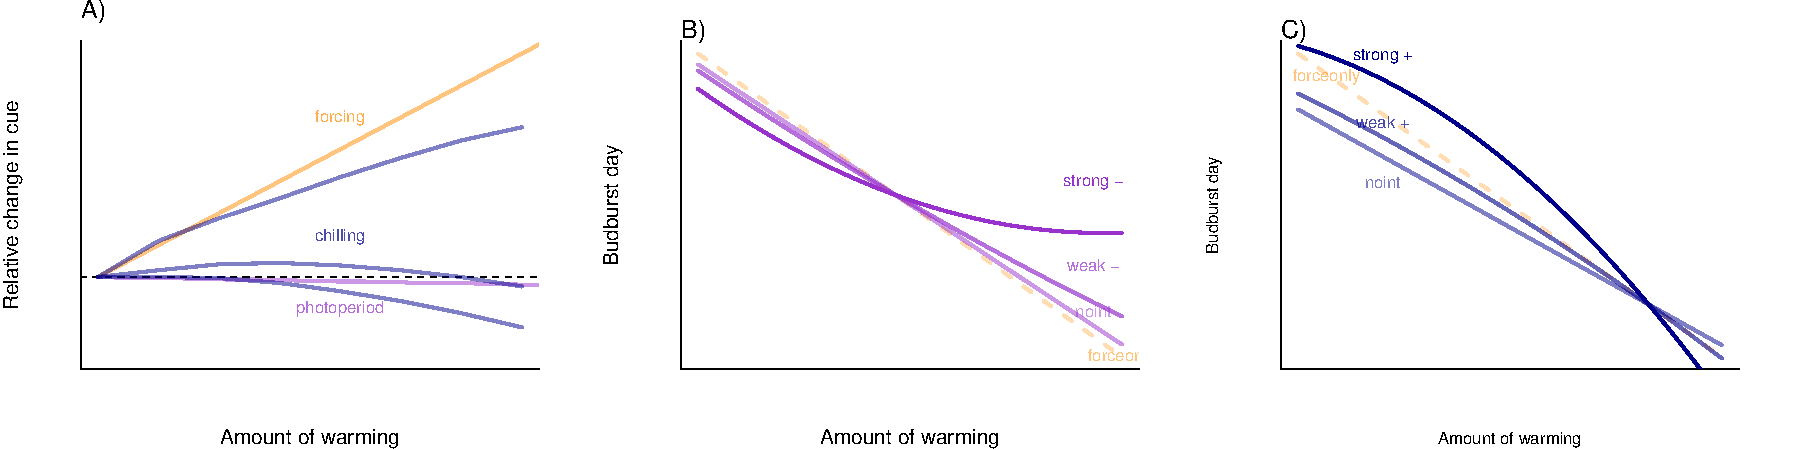
\includegraphics[width=1\textwidth]{..//..//analyses/limitingcues/figures/intxnsims2021photoaltwithchill_3panels.pdf} % intxnsims2021photoaltwithchill_6panels_polyg_imc.png
\caption{Interactions are unlikely to produce nonlinearities unless there are correlated shifts in cues, which may occur with climate change. Much research focuses on how warming increases forcing, but warming may also alter other cues, including photoperiod experienced near the time of the event, which is expected to shorten, and chilling, which may either increase or decrease (A). Shifts in forcing alongside shifts in a second cue may produce non-linearities due to the interaction between cues (B-C) showing the effect of: forcing-only in yellow, both cues without an interaction in lighter purple/blue, and both cues with an interaction in darker purple/blue). The overall change in budburst day predicted with warming depends on the sign of the second cue (negative in B, positive in C), as well as its strength (weak/strong).}
  \label{fig:intxncues}
\end{figure}
% Here we show examples considering a forcing x photoperiod interaction (top) and forcing x chilling (bottom), with both a linear effect of photoperiod or chilling (middle panels) or a threshold effect (left panels) versus an effect of forcing only (dashed gray line). These non-linearities come from the levels of both cues shifting at once: for the photoperiod example (top), as temperatures rise, forcing increases and the photoperiod experienced near the time of the event shortens (a similar response would be seen for lowering chilling), while for the chilling example (bottom), as temperatures rise forcing and chilling increases.}

\clearpage
\begin{figure}
\centering
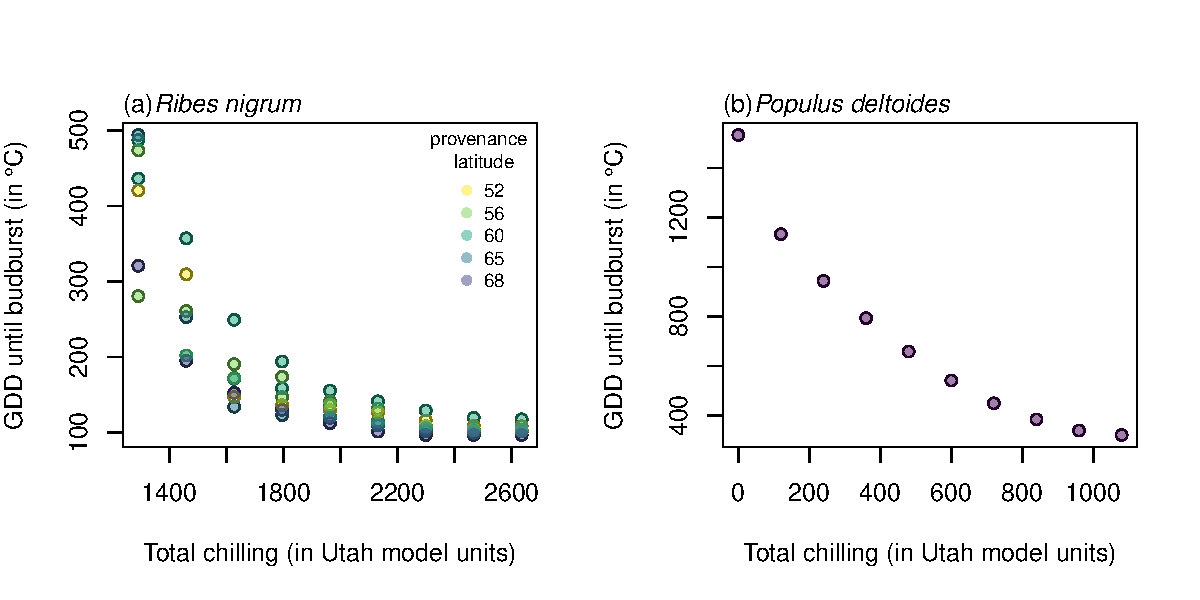
\includegraphics[width=1\textwidth]{..//..//analyses/limitingcues/figures/gddbyutahpretty.pdf}
\caption{A common example of how the level of one cue can modify the required level of another cue comes from experiments finding that the amount of chilling affects the amount of forcing needed for budburst. Here, we show this from experiments in black currant (\emph{Ribes nigrum}) from \citet{Sonsteby:2014aa} and eastern cottonwood (\emph{Populus deltoides}) from \citet{Thielges:1976aa}. Forcing is estimated as growing degree days (GDD, sum of temperatures $>0\degree$C) while chilling is estimated using the Utah Model \citep[see][]{richardson1974}.} % \citet{Cronje:2003aa} which studied apple (\emph{Malus sylvestris}), 
  \label{fig:gddbyutah} 
\end{figure}
% GDD_plottinglimcues.R


\clearpage
\begin{figure}[t!]
\centering
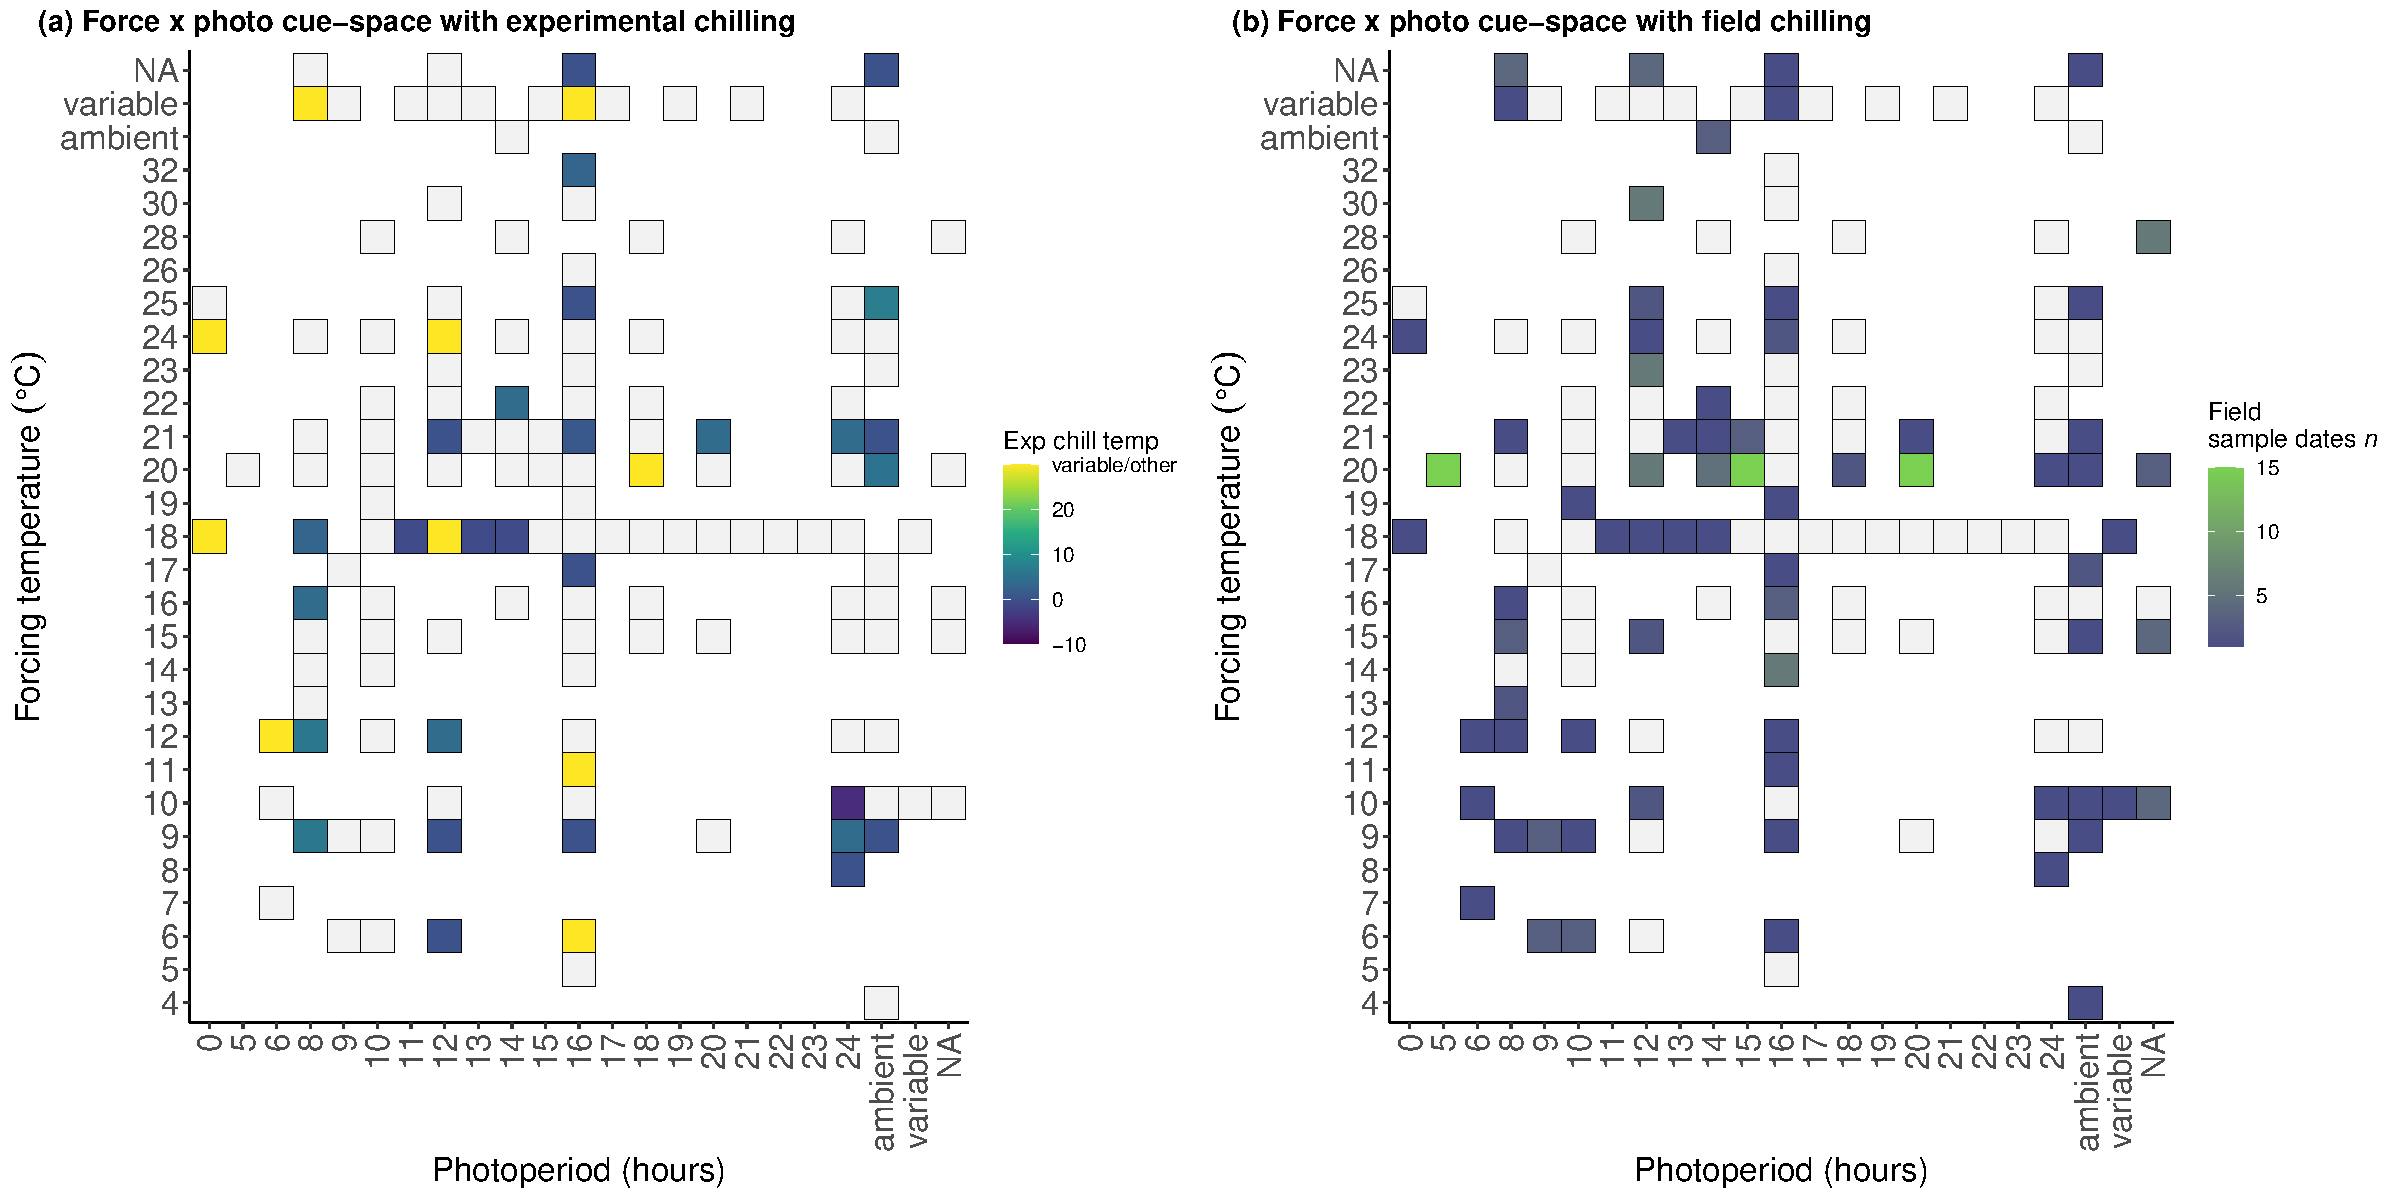
\includegraphics[width=1.1\textwidth]{..//..//analyses/limitingcues/figures/heatmapphotoxforcexchill2panel.pdf}
\caption{Studies have examined a range of cue-space (forcing temperature x photoperiod across two methods to manipulate chilling: a) experimentally or b) using multiple field sampling dates), but a focus on certain levels of cues and limited reporting of all cues makes using these data to estimate non-linearities challenging (see `Forecasting non-linear responses: Do we have the necessary data?'). Gray squares indicate a combination of forcing x photoperiod not present for that method of chilling design (includes studies that did not clearly define chilling treatments), while a value of `NA' indicates that we could not estimate a level of a particular cue because it was not clearly reported.  Photoperiod treatments were generally only applied (or reported) during forcing conditions.}
  \label{fig:heatmaps} 
\end{figure}

\clearpage

\begin{figure}[t!]
\centering
\includegraphics[width=1\textwidth]{figures/Fig7_noblues_densities.png}
\caption{Comparison of differences in experimental treatments and predicted temperature changes in the future for each of two species: \emph{Fagus sylvatica} (A-B) and \emph{Betula pendula}. Points represent a site with spring phenology data  \citep[from the PEP725 database,][]{Templ2018} and show the predicted change (2080s average - 1970s average) in minimum (A,C) and maximum (B,D) temperatures 60 days before leafout. We found that treatment differences (see lines in inlay plots, green lines show the treatments for that exact species, while black lines show across all species) generally bracketed predicted changes (histograms in inlay plots show the same predicted changes in temperature represented also by the mapped points), but were on average much larger in magnitude. We show chilling (A, C) and forcing (B, D) differences in treatments across studies (for \emph{Fagus sylvatica} there are no chilling treatments of differing temperatures). For more details, see `Comparing experimental treatments to forecasted trends' in the Supporting Information.}
\label{fig:pep} % studydesignplots.R
\end{figure}

\end{document}
